\documentclass[11pt, a4paper]{article}
\usepackage{pdfpages}
\usepackage{parallel}
\usepackage[T2A]{fontenc}
\usepackage{ucs}
\usepackage[utf8x]{inputenc}
\usepackage[polish,english,russian]{babel}
\usepackage{hyperref}
\usepackage{rotating}
\usepackage[inner=2cm,top=1.8cm,outer=2cm,bottom=2.3cm,nohead]{geometry}
\usepackage{listings}
\usepackage{graphicx}
\usepackage{wrapfig}
\usepackage{longtable}
\usepackage{indentfirst}
\usepackage{array}
\usepackage{tikzsymbols}
\usepackage{soul}
\usepackage[ruled,vlined]{algorithm2e}
%\counterwithout{figure}{section} 

\usepackage{url}
\makeatletter
\g@addto@macro{\UrlBreaks}{\UrlOrds}
\makeatother

\newcolumntype{P}[1]{>{\raggedright\arraybackslash}p{#1}}
\frenchspacing
\usepackage{fixltx2e} %text sub- and superscripts
\usepackage{icomma} % коскі ў матэматычным рэжыме
\PreloadUnicodePage{4}

\newcommand{\longpage}{\enlargethispage{\baselineskip}}
\newcommand{\shortpage}{\enlargethispage{-\baselineskip}}

\def\switchlang#1{\expandafter\csname switchlang#1\endcsname}
\def\switchlangbe{
\let\saverefname=\refname%
\def\refname{Літаратура}%
\def\figurename{Іл.}%
}
\def\switchlangen{
\let\saverefname=\refname%
\def\refname{References}%
\def\figurename{Fig.}%
}
\def\switchlangru{
\let\saverefname=\refname%
\let\savefigurename=\figurename%
\def\refname{Литература}%
\def\figurename{Рис.}%
}

\hyphenation{admi-ni-stra-tive}
\hyphenation{ex-pe-ri-ence}
\hyphenation{fle-xi-bi-li-ty}
\hyphenation{Py-thon}
\hyphenation{ma-the-ma-ti-cal}
\hyphenation{re-ported}
\hyphenation{imp-le-menta-tions}
\hyphenation{pro-vides}
\hyphenation{en-gi-neering}
\hyphenation{com-pa-ti-bi-li-ty}
\hyphenation{im-pos-sible}
\hyphenation{desk-top}
\hyphenation{elec-tro-nic}
\hyphenation{com-pa-ny}
\hyphenation{de-ve-lop-ment}
\hyphenation{de-ve-loping}
\hyphenation{de-ve-lop}
\hyphenation{da-ta-ba-se}
\hyphenation{plat-forms}
\hyphenation{or-ga-ni-za-tion}
\hyphenation{pro-gramming}
\hyphenation{in-stru-ments}
\hyphenation{Li-nux}
\hyphenation{sour-ce}
\hyphenation{en-vi-ron-ment}
\hyphenation{Te-le-pathy}
\hyphenation{Li-nux-ov-ka}
\hyphenation{Open-BSD}
\hyphenation{Free-BSD}
\hyphenation{men-ti-on-ed}
\hyphenation{app-li-ca-tion}

\def\progref!#1!{\texttt{#1}}
\renewcommand{\arraystretch}{2} %Іначай формулы ў матрыцы зліпаюцца з лініямі
\usepackage{array}

\def\interview #1 (#2), #3, #4, #5\par{

\section[#1, #3, #4]{#1 -- #3, #4}
\def\qname{LVEE}
\def\aname{#1}
\def\q ##1\par{{\noindent \bf \qname: ##1 }\par}
\def\a{{\noindent \bf \aname: } \def\qname{L}\def\aname{#2}}
}

\def\interview* #1 (#2), #3, #4, #5\par{

\section*{#1\\{\small\rm #3, #4. #5}}
\ifx\ParallelWhichBox\undefined%
    \addcontentsline{toc}{section}{#1, #3, #4}%
\else%
\ifnum\ParallelWhichBox=0%
    \addcontentsline{toc}{section}{#1, #3, #4}%
\fi\fi%

\def\qname{LVEE}
\def\aname{#1}
\def\q ##1\par{{\noindent \bf \qname: ##1 }\par}
\def\a{{\noindent \bf \aname: } \def\qname{L}\def\aname{#2}}
}

\newcommand{\interviewfooter}[1]{
\vskip 1em
\noindent \textit{#1}
}

\switchlang{ru}
\begin{document}

\title{1988 "--- Tandy TRS-80 Deluxe Mouse}
\date{}
\maketitle
\selectlanguage{russian}
Мышь Tandy TRS-80 Deluxe Mouse (рис. \ref{fig:TandyDeluxeMousePic}) "--- вторая из двух мышей, разработанных для компьютеров RadioShack TRS-80 Color Computer (позднее переименованным в Tandy Color Computer). Color Computer model 1, выпущенный в 1981 году, представлял собой домашний компьютер, оснащенный резиновой клавиатурой как у микрокалькуляторов, имевший ОЗУ от 4Кб до 32Кб, 8-битную разрядность машинного слова и использовал телевизор в качестве дисплея \cite{wiki}. С течением времени список периферийных устройств расширялся, в 1984 году в их список добавилась мышь Color Mouse, а в 1988 году "--- Deluxe Mouse \cite{adv}. Обе мыши производилась по контракту японской компанией Alps и подключались в порт аналогового джойстика.

\begin{figure}[h]
    \centering
    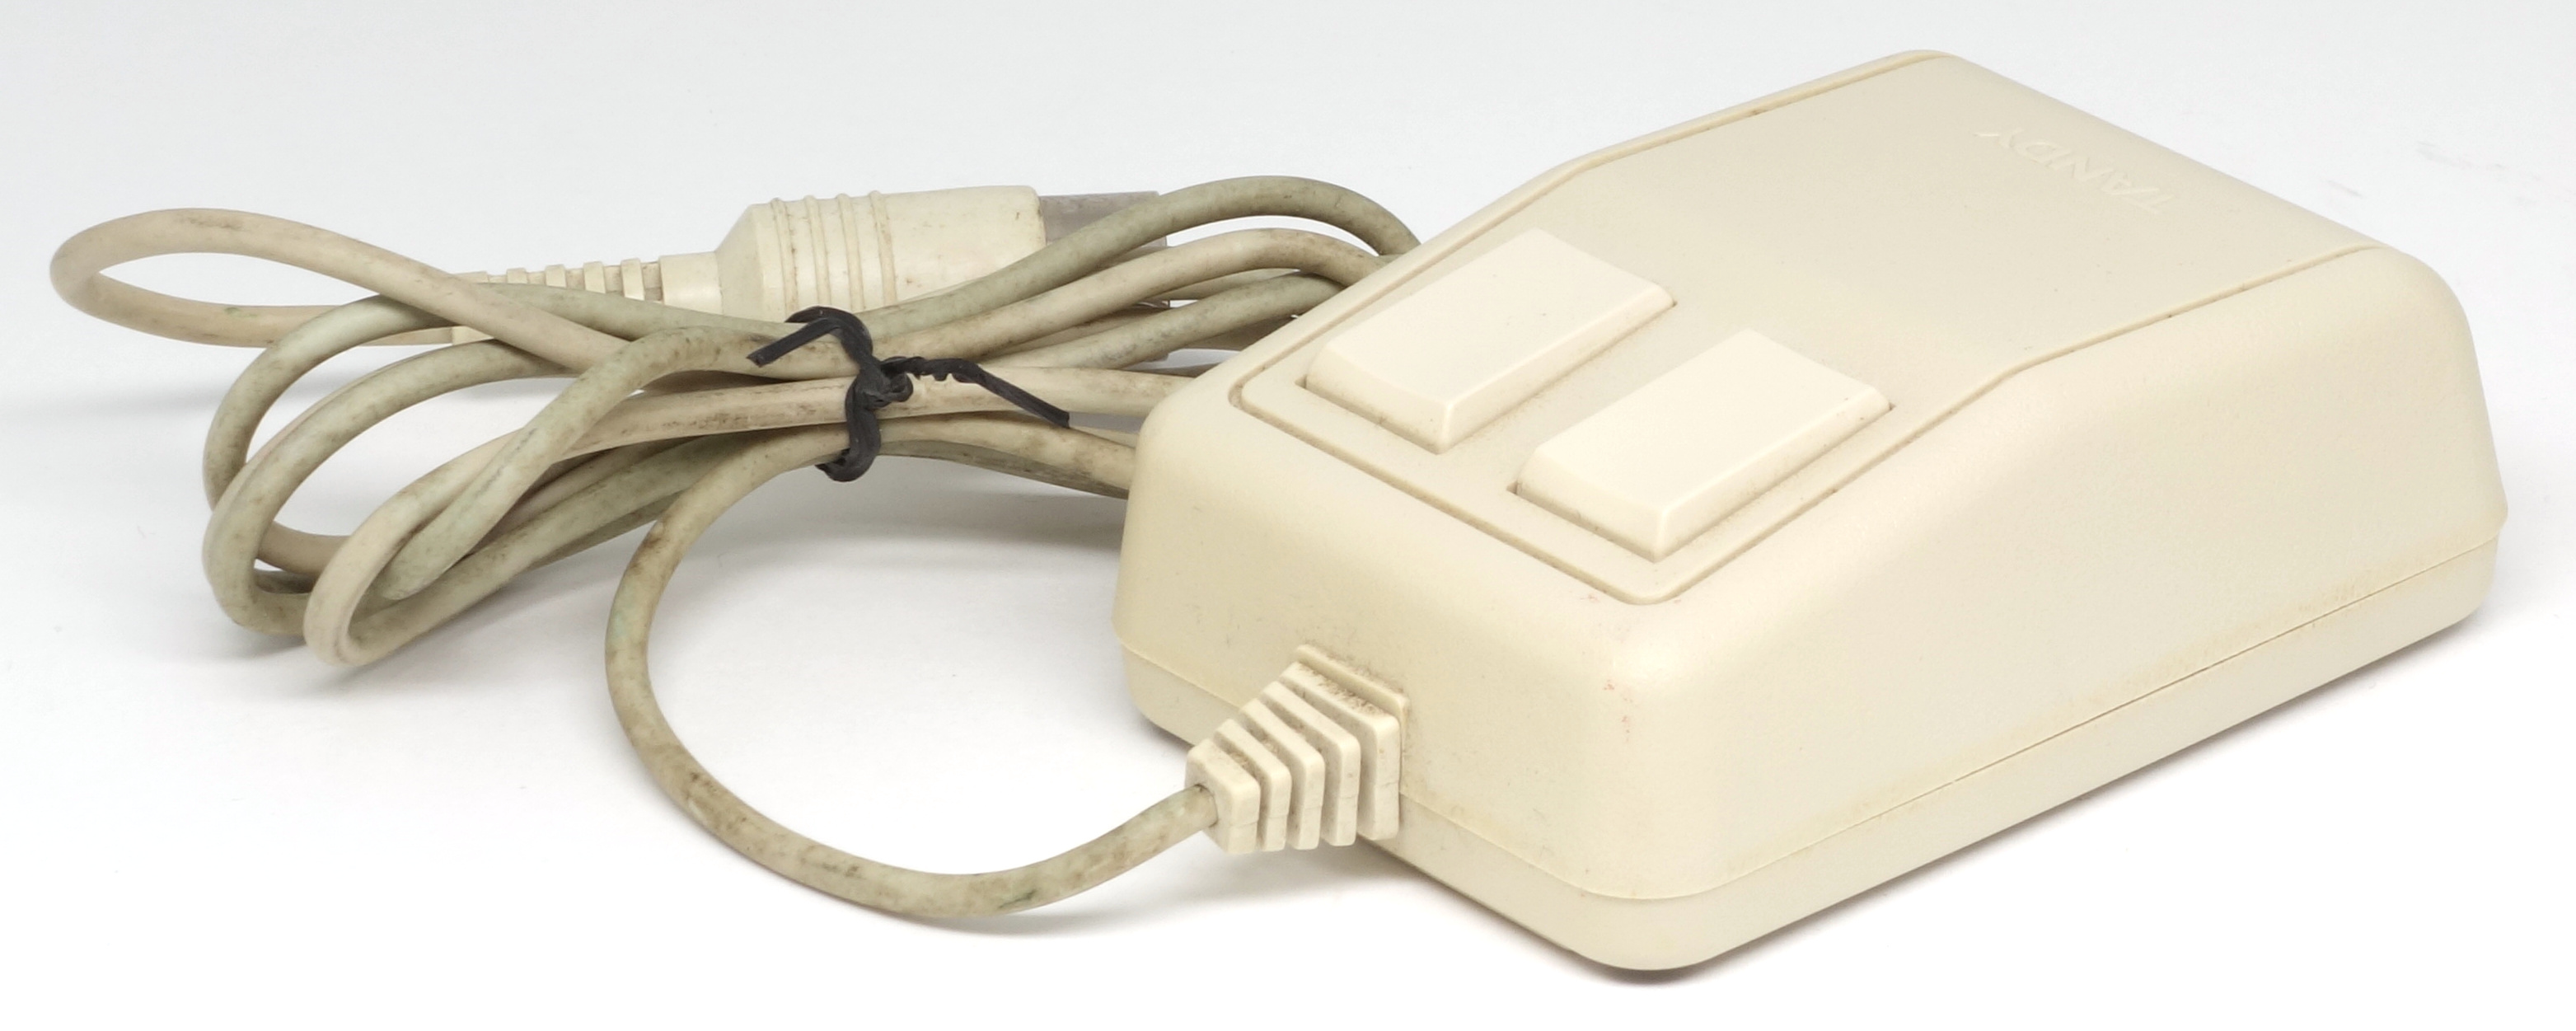
\includegraphics[scale=0.7]{1988_tandy_trs80_deluxe_mouse/pic_30.jpg}
    \caption{Tandy Deluxe Mouse}
    \label{fig:TandyDeluxeMousePic}
\end{figure}

\begin{figure}[h]
    \centering
    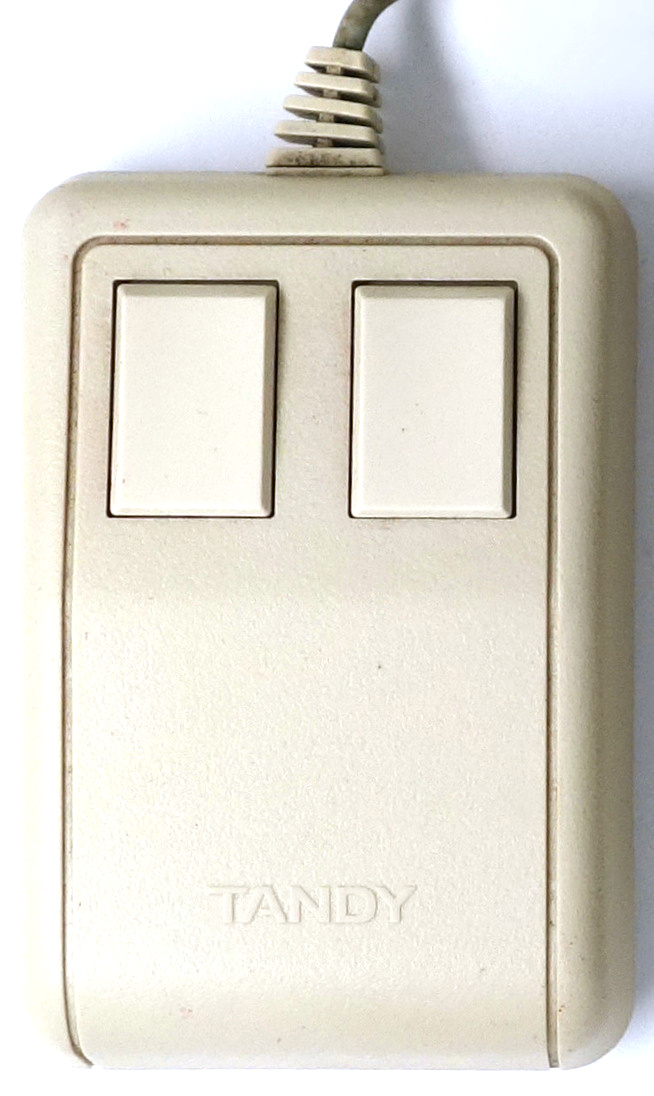
\includegraphics[scale=0.65]{1988_tandy_trs80_deluxe_mouse/top_60.jpg}
    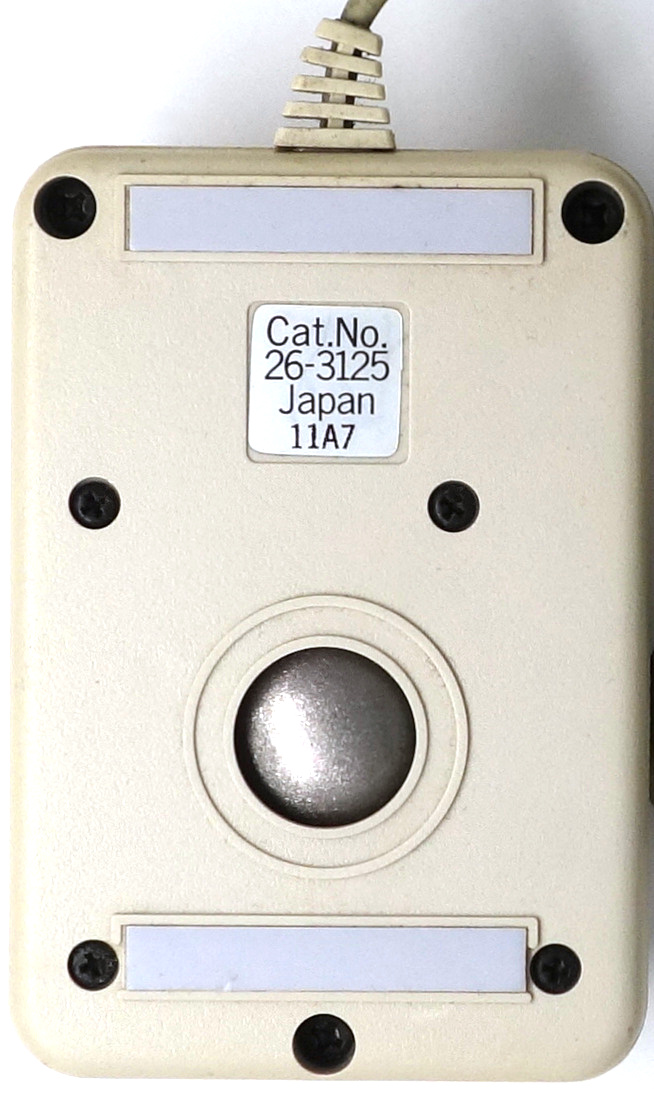
\includegraphics[scale=0.65]{1988_tandy_trs80_deluxe_mouse/bottom_30.jpg}
    \caption{Tandy Deluxe Mouse, вид сверху и снизу}
    \label{fig:TandyDeluxeMouseTopAndBottom}
\end{figure}

В отличие от своей предшественницы Color Mouse, мышь Tandy TRS-80 Deluxe Mouse имеет две кнопки (рис. \ref{fig:TandyDeluxeMouseTopAndBottom}) и бежевый корпус, достаточно типичный для мышей 80-х годов \cite{hierophant}.

Нижняя сторона корпуса демонстрирует точно такой же как у Color Mouse стальной шар и такое же отсутствие съемного кольца, позволяющего извлечь шар для чистки. Усовершенствованием является появление накладок из низкофрикционного материала, облегчающих скольжение мыши.

Мышь имеет небольшие размеры, также типичные для 80-х годов, и довольно высокий корпус (рис. \ref{fig:TandyDeluxeMouseSize}).

\begin{figure}[h]
    \centering
    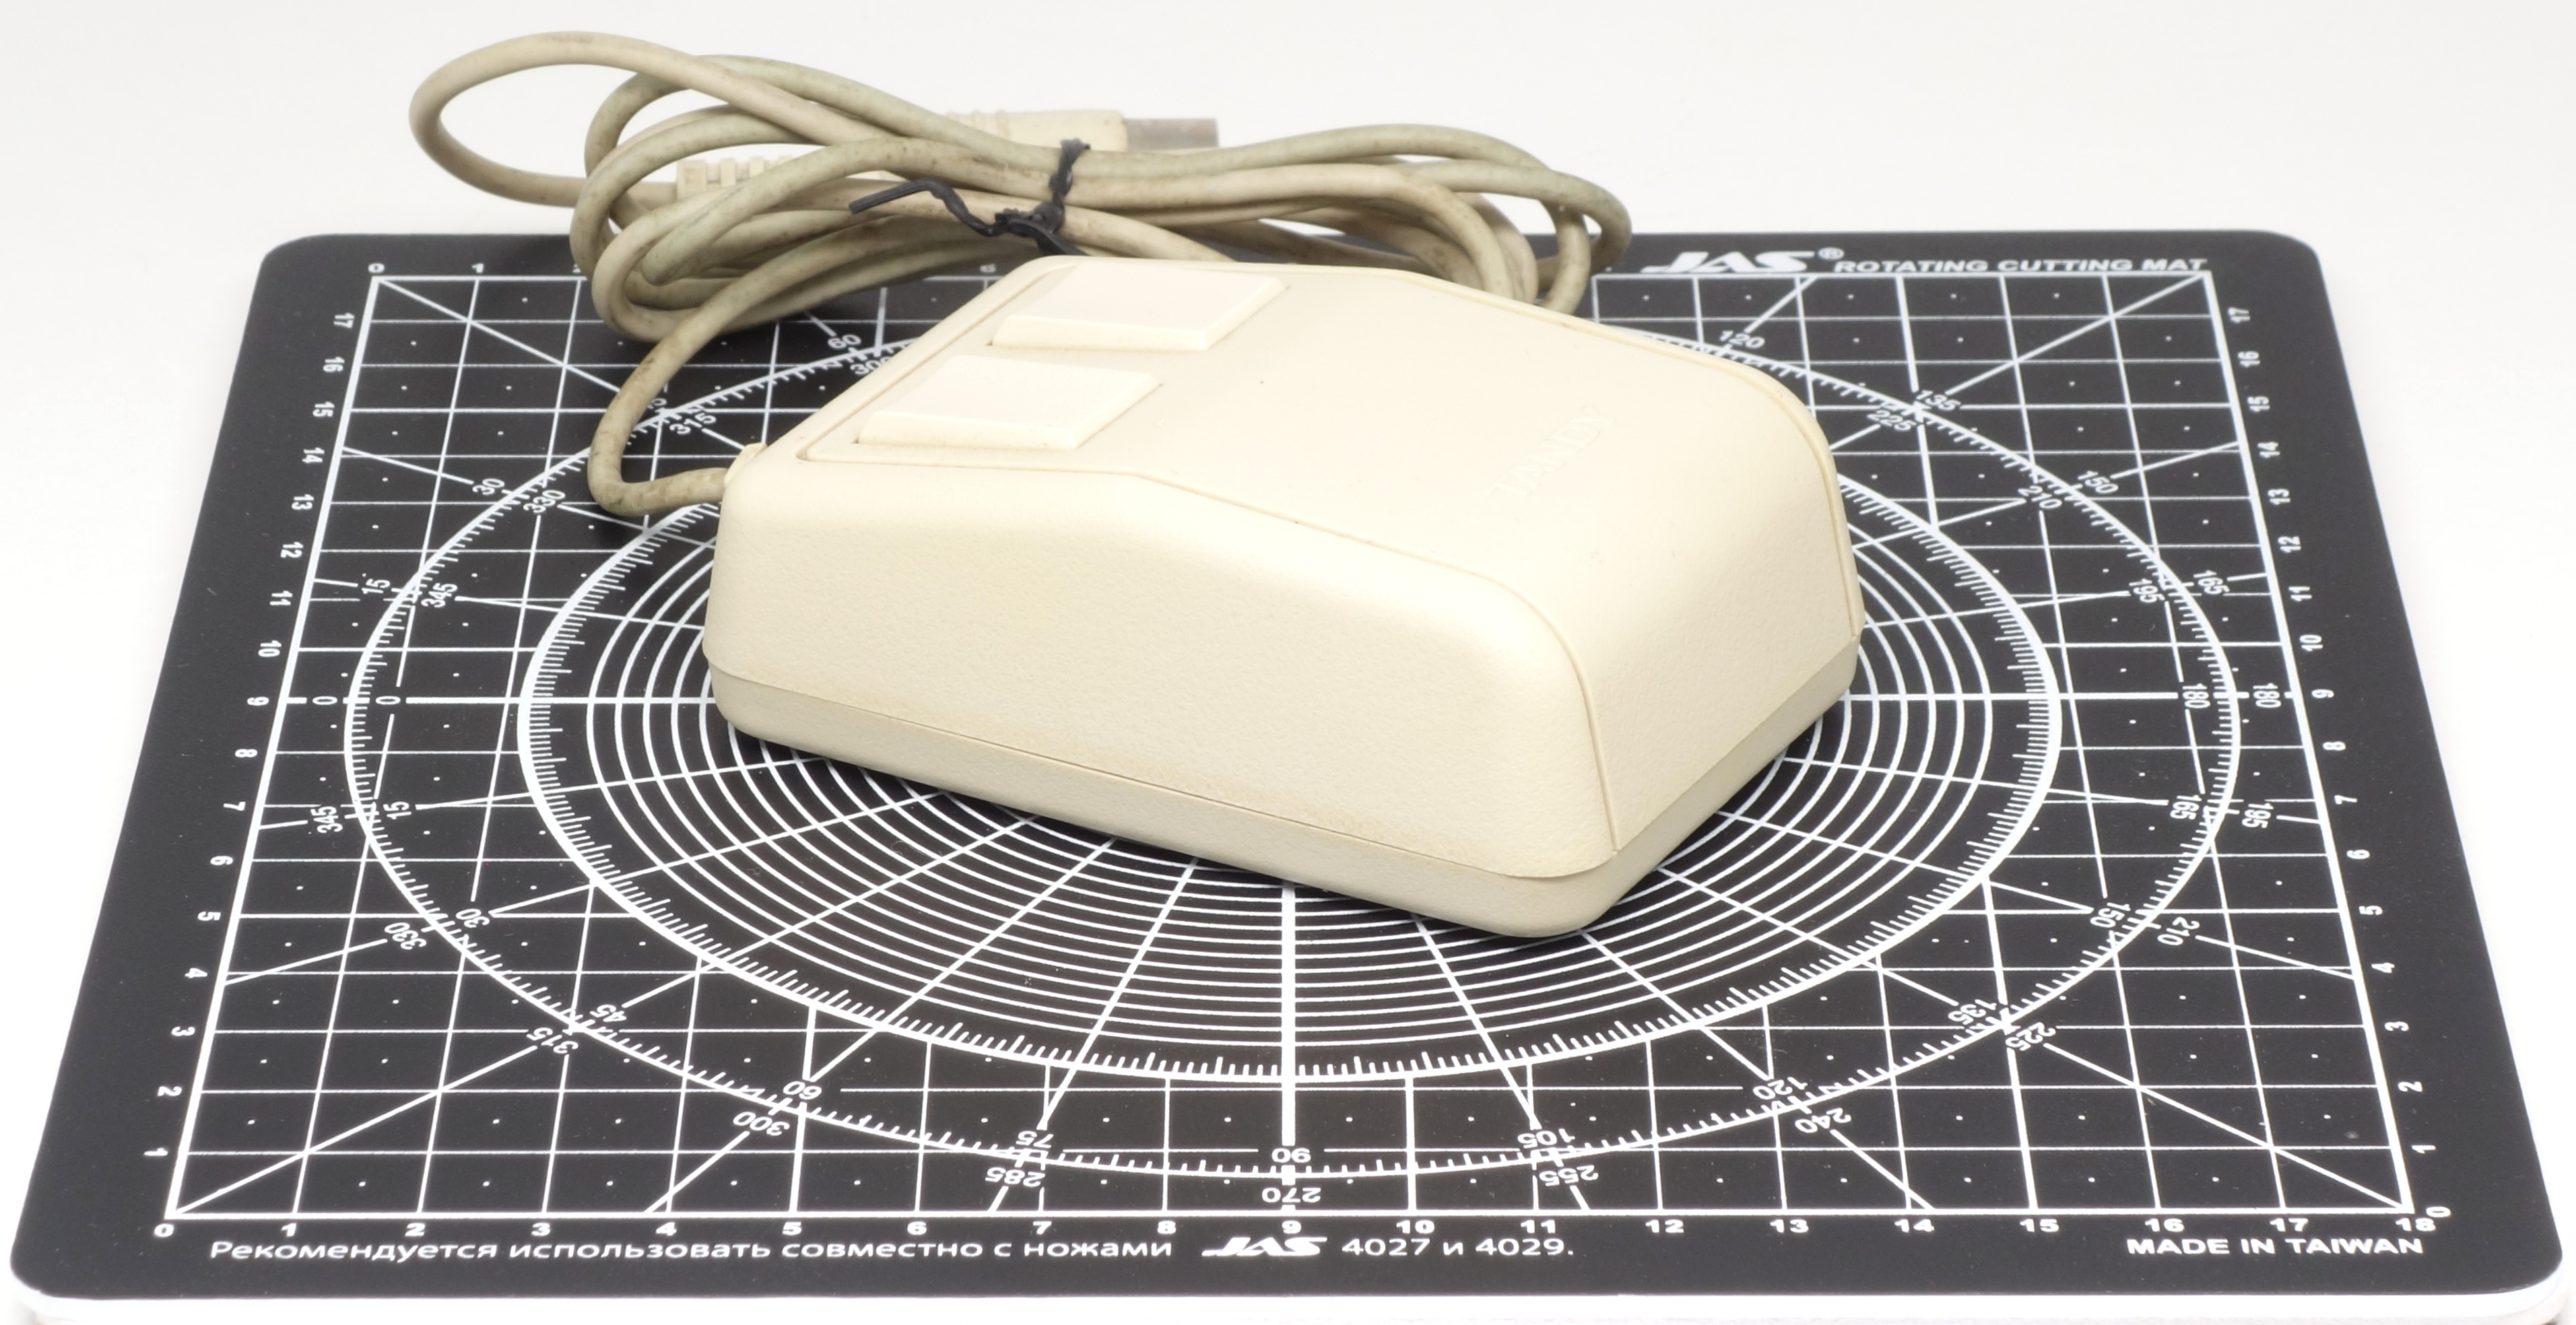
\includegraphics[scale=0.49]{1988_tandy_trs80_deluxe_mouse/size_15.jpg}
    \caption{Tandy Deluxe Mouse на размерном коврике с шагом сетки 1~см}
    \label{fig:TandyDeluxeMouseSize}
\end{figure}

Кнопки Deluxe Mouse имеют достаточно большую площадь и небольшой прогиб, что обеспечивает их достаточно комфортное нажатие пальцами (рис. \ref{fig:TandyDeluxeMouseHand}). В целом, закругленные ребра корпуса оказывают некоторое положительное влияние на эргономику, однако типичная для мышей 80-х годов форма корпуа не предоставляет никакой существенной опоры для ладони.

\begin{figure}[h]
    \centering
    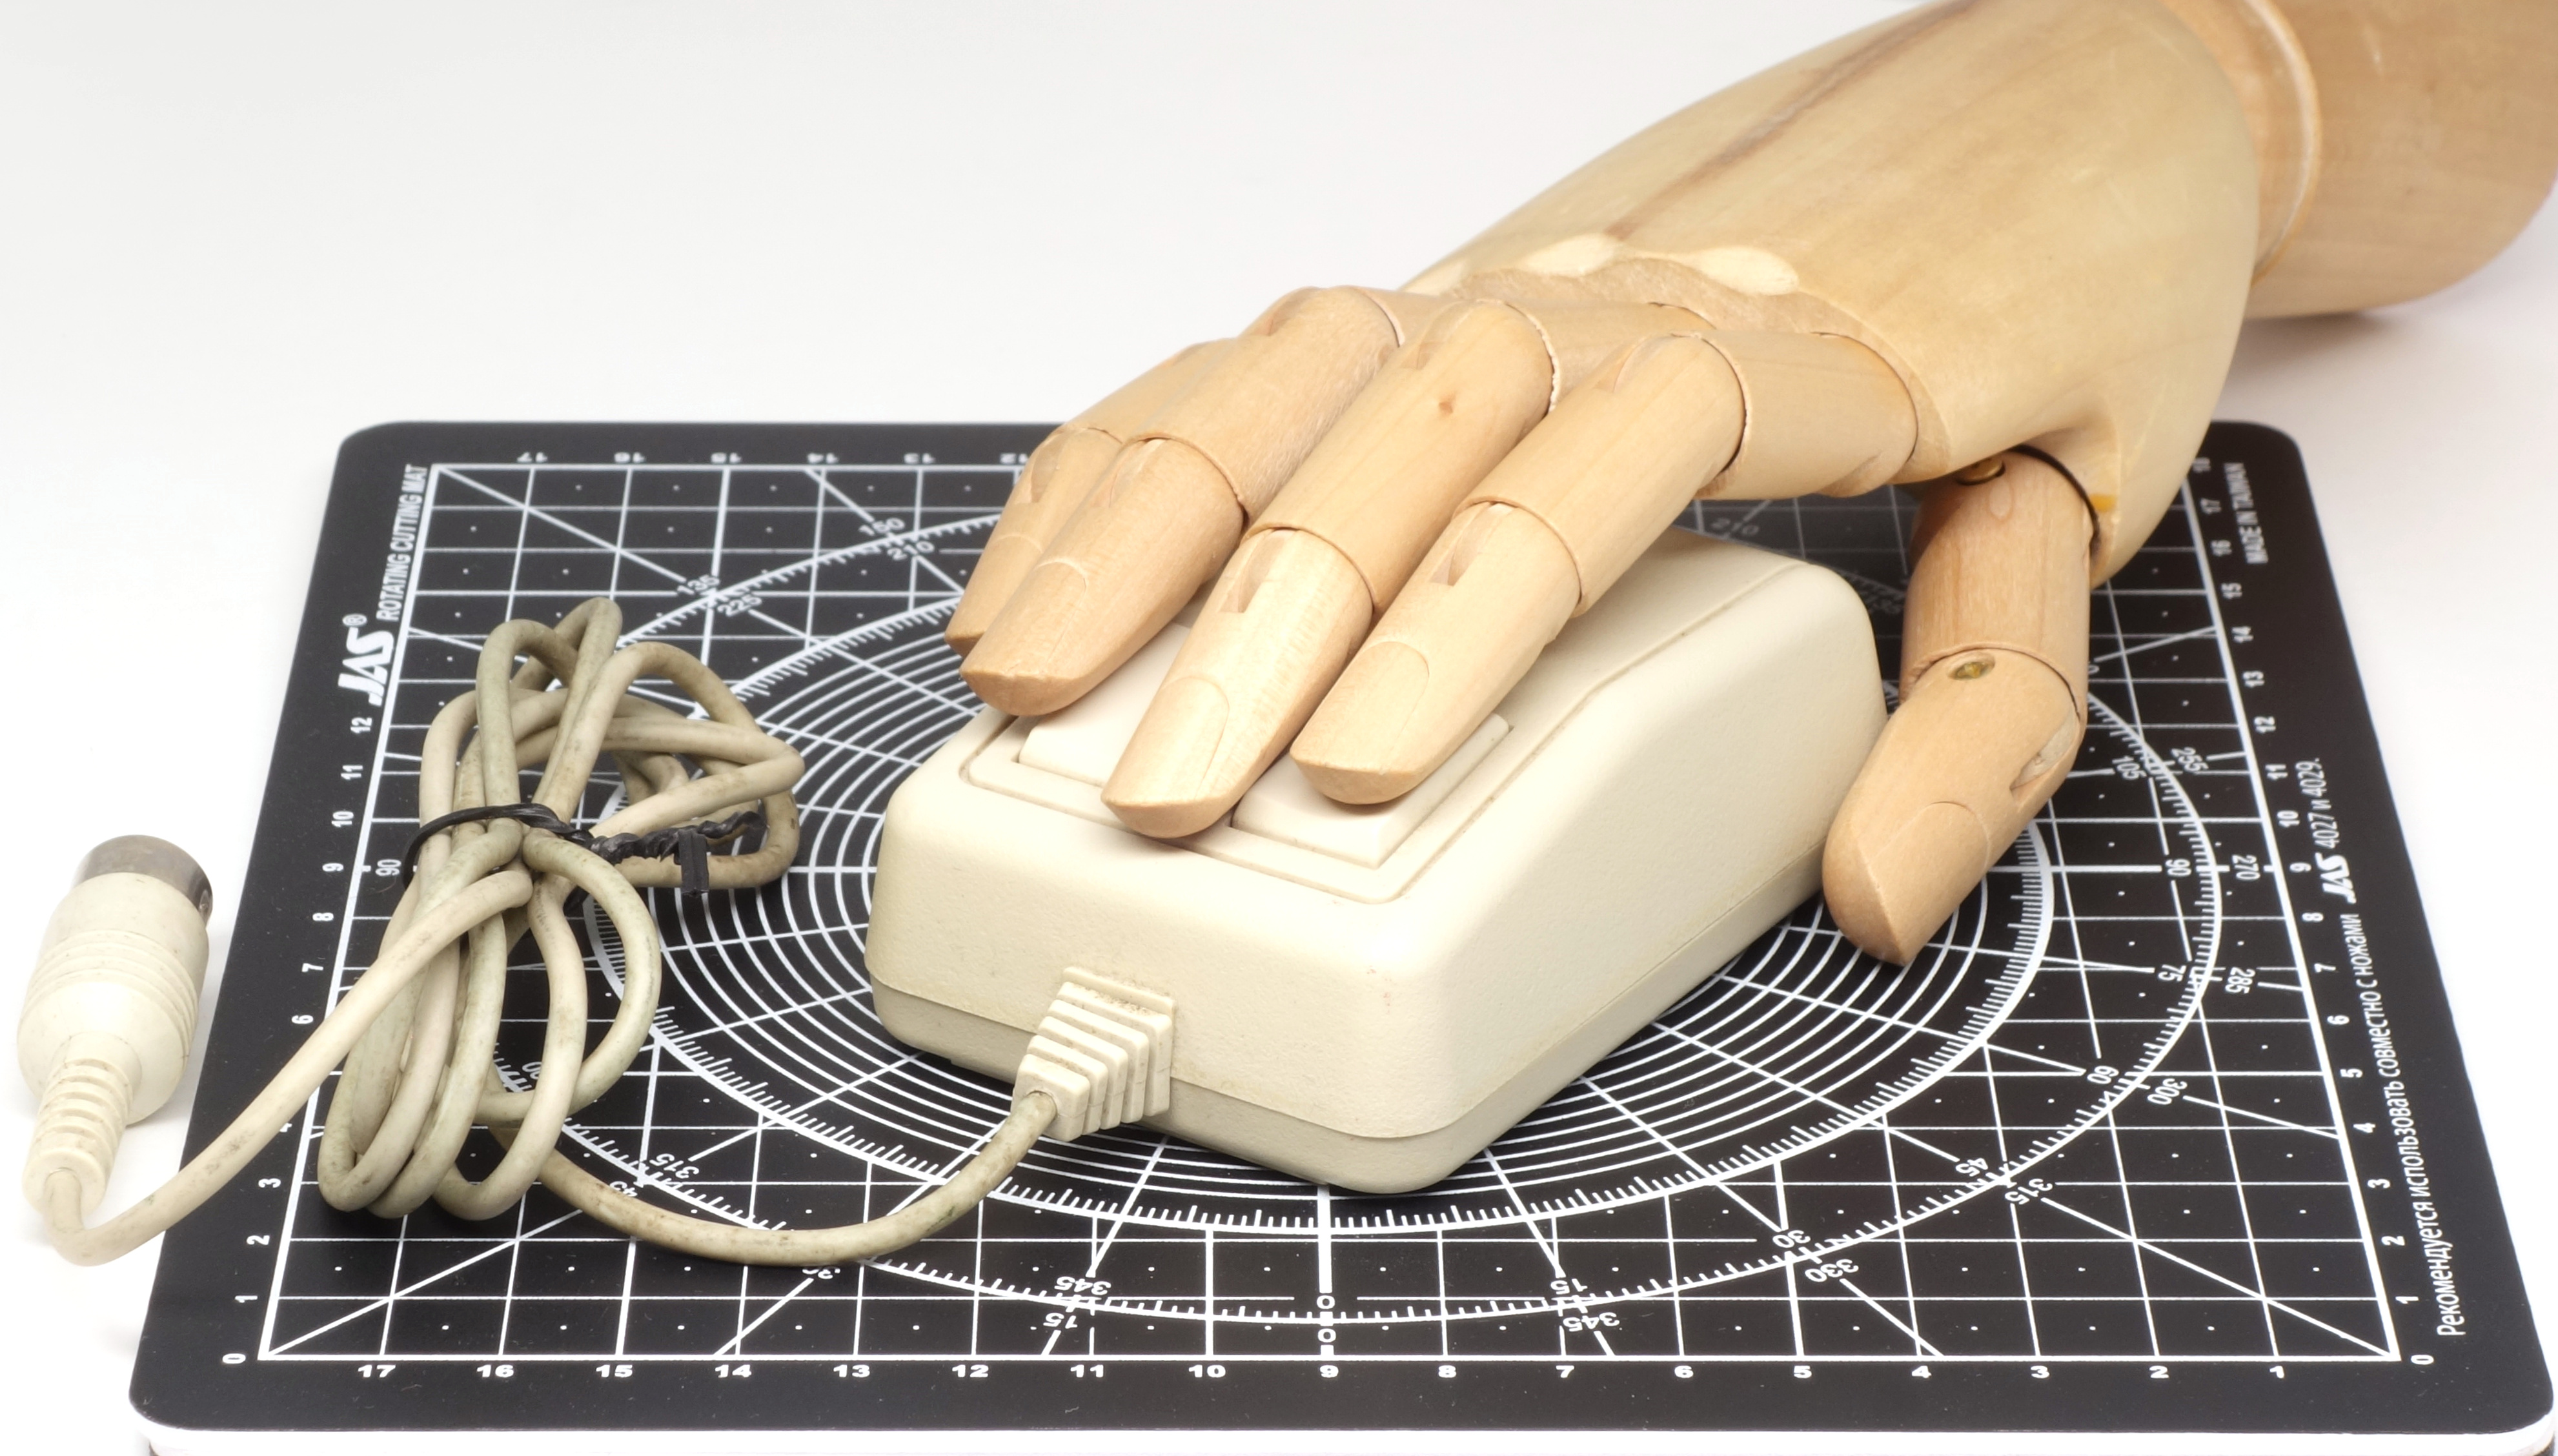
\includegraphics[scale=0.55]{1988_tandy_trs80_deluxe_mouse/hand_15.jpg}
    \caption{Tandy Deluxe Mouse с моделью руки человека}
    \label{fig:TandyDeluxeMouseHand}
\end{figure}

Как упоминалось, мышь подключается к порту аналогового джойстика. Как и в случае джойстика, информация о каждой из двух координат закодирована в аналоговом виде, величиной электрического напряжения на соответствующем контакте разъема. Как и Color Mouse, данная мышь имеет разрешение в 64 <<шага>> по каждой из координатных осей \cite{manual}, очевидно связанное ограниченными возможностями аналогово-цифрового преобразователя Tandy Color Computer; драйвера, позволяющие использовать аналоговый джойстик для перемещения курсора мыши, также демонстрируют малую точность позиционирования \cite{hierophant}.

\begin{figure}[h]
    \centering
    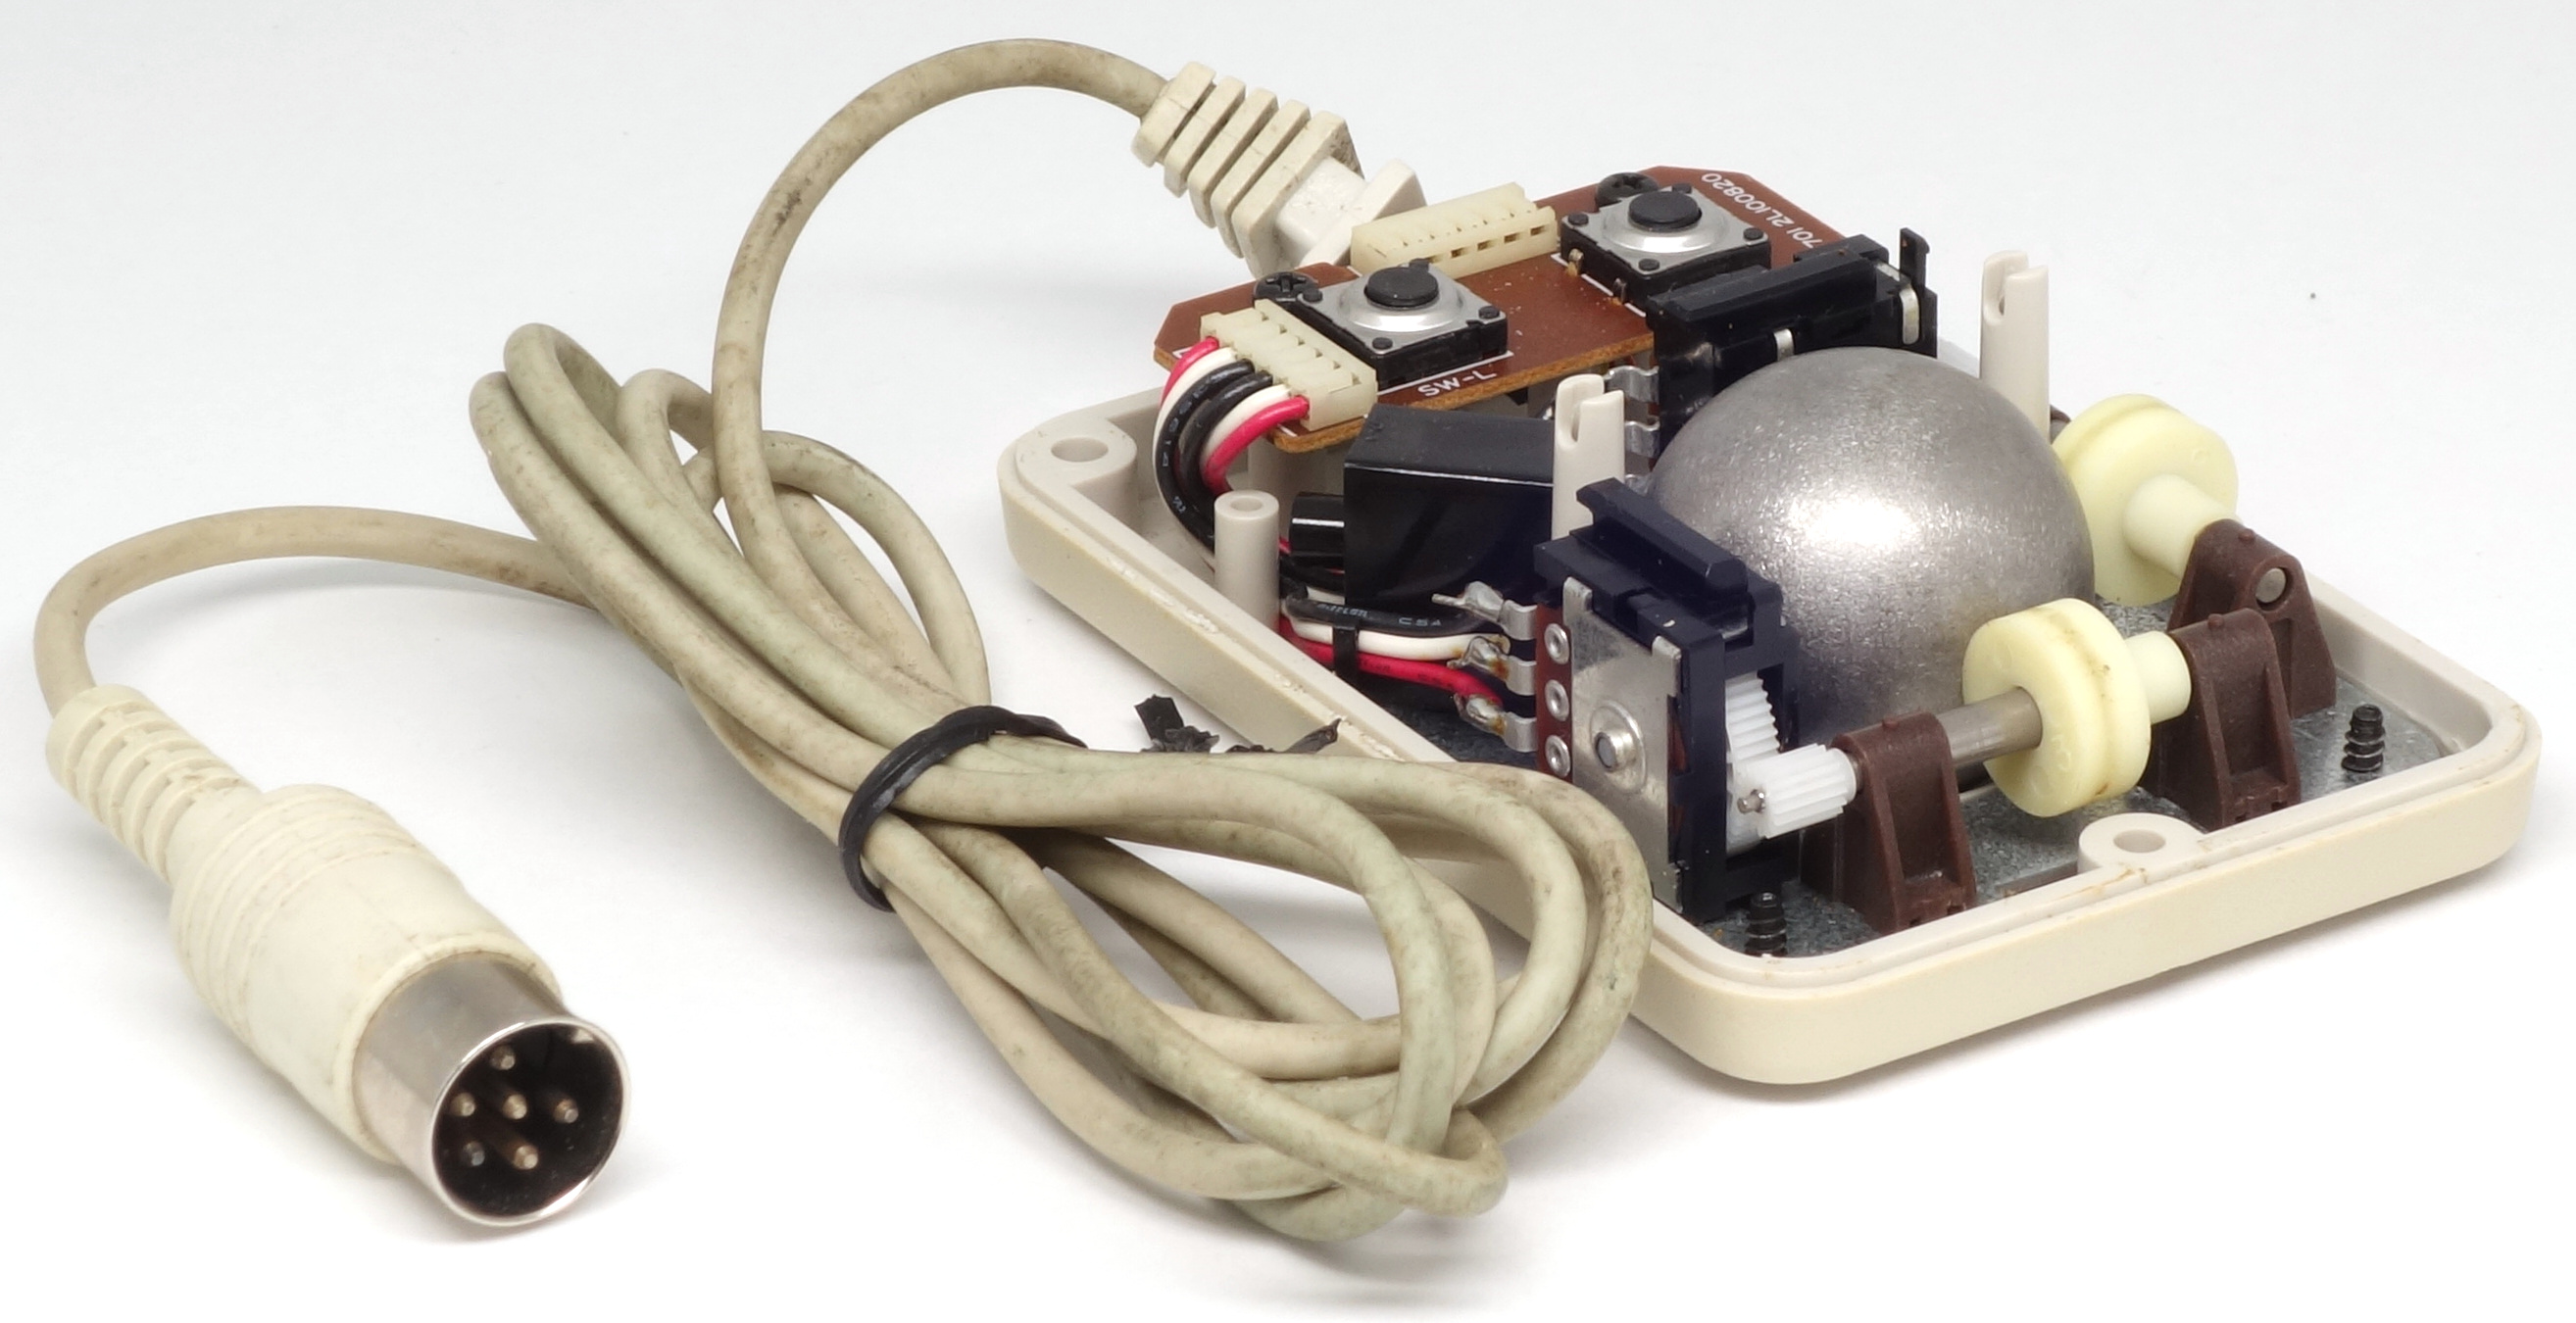
\includegraphics[scale=0.8]{1988_tandy_trs80_deluxe_mouse/inside_30.jpg}
    \caption{Tandy Deluxe Mouse в разобранном виде}
    \label{fig:TandyDeluxeMouseInside}
\end{figure}

В разобранном виде манипулятор показан на рис. \ref{fig:TandyDeluxeMouseInside}. Как и Color Mouse, мышь Tandy Deluxe не использует контактные или оптомеханические энкодеры: вместо этого шар передает движение паре потенциометров точно так же, как это делает рукоятка аналогового джойстика. Безусловно, такое решение имеет существенные недостатки: мышь не имеет возможностей калибровки, также в отличие от джойстика не существует способа определить по виду мыши, что ее потенциометры переведены в среднее положение, которому должно соответствовать расположение мыши в центре коврика, или что они достигли крайнего положения. Однако, поскольку Tandy Deluxe Mouse представляет собой манипулятор с абсолютными координатами, пользователь может оценить положение курсора на экране и поместить мышь на часть коврика, приблизительно соответствующую этому положению.

\begin{thebibliography}{9}
\bibitem {wiki} TRS-80 Color Computer -- Wikipedia \url{https://en.wikipedia.org/wiki/TRS-80_Color_Computer}
\bibitem {adv} 1988 Radio Shack Catalog. p. 177 \url{https://www.radioshackcatalogs.com/flipbook/1988_radioshack_catalog.html}, \url{https://web.archive.org/web/20210331035502/https://www.radioshackcatalogs.com/flipbook/catalogs/main/1988/177.jpg}
\bibitem {hierophant} Tandy Color Computer Mice - A Viable Alternative for Tandy 1000s without a Serial Port? January 21, 2016. -- \url{http://nerdlypleasures.blogspot.com/2016/01/tandy-color-computer-mice-viable.html}
\bibitem {manual} TANDY  COLOR COMPUTER TANDY 1000 SX / 1000 EX COLOR MOUSE Operational Manual \url{https://colorcomputerarchive.com/repo/Documents/Manuals/Hardware/Deluxe%20Color%20Mouse%20%28Tandy%29.pdf}
\end{thebibliography}
\end{document}
